\section{Abstract}\label{abstract}

We compare three covariance estimators --- raw sample covariance,
Ledoit--Wolf shrinkage, and Marchenko--Pastur (MP) eigenvalue clipping
(Laloux--Bouchaud-- Potters) --- inside a walk-forward
global-minimum-variance backtest on factor-model panels, across three
\(N/T\) regimes and five seeds. The ranking reproduces the
random-matrix-theory thesis: at low \(N/T\) all estimators converge; at
\(N/T = 0.5\), MP-clipped and LW covariances beat the sample estimator
by \(\approx 0.5\) net Sharpe with paired-bootstrap intervals excluding
zero. We document two measurement traps that silently dominate naive
implementations: panel-drift contamination of cross-method comparisons
(fixed by return demeaning) and the Jensen gap between simple and log
returns in cumulative-price panels.

\section{1. Setup}\label{setup}

\textbf{Estimators.} Given trailing returns
\(R \in \mathbb{R}^{T \times N}\) and correlation eigenvalues
\(\lambda_1 \ge \dots \ge \lambda_N\):

\begin{itemize}
\tightlist
\item
  \emph{sample}: \(S = R^\top R / (T-1)\);
\item
  \emph{Ledoit--Wolf}: optimal shrinkage of \(S\) toward \(\mu I\);
\item
  \emph{MP clipping}: fit noise level \(\sigma^2\) by bisection on the
  bulk-mean consistency condition, compute the MP edge
  \(\lambda_+ = \sigma^2(1 + \sqrt{q})^2\) with \(q = N/T\), replace
  every eigenvalue below the edge by their average (noise directions
  carry no information), keep outliers, restore trace.
\end{itemize}

\textbf{Backtest.} Every 21 days, weights solve the long-only GMV
problem from a strictly trailing 250-day window; realized next-period
returns accrue at 5 bps cost on turnover. Three panels from a
\(k\)-factor DGP (\(\sigma_{\text{idio}} = 1.5\%\)/day): (100, 1000),
(100, 400), (200, 400) days; five seeds each.

\textbf{Controls.} Per-asset mean returns are removed over the full
sample. This leaks the mean (only) into the backtest and is deliberate:
with arbitrary panel drift, cross-method Sharpe differences are
dominated by drift noise rather than covariance quality. The covariance
matrix itself is always estimated on strictly past data.

\section{2. The two measurement traps}\label{the-two-measurement-traps}

\textbf{Trap 1: panel drift.} A zero-\emph{expected}-mean DGP still
produces realized cross-sectional drift with cross-seed dispersion of
\(\pm 2.7\) Sharpe at 2\% annualized volatility --- three times larger
than the estimator effects under study. Without demeaning, the
comparison is a random-number generator.

\textbf{Trap 2: Jensen gap.} Cumulative-price panels
\(P = 100\prod(1 + r)\) carry log returns with mean
\(- \sigma^2/2 \approx
-6.7\%\)/yr at these volatilities. Any long-only portfolio eats a
weighted share of this drift; a permutation null (shuffled asset
timelines) still showed \(-7\sigma\) mean ``alpha'', proving the
artifact was mechanical. A related implementation subtlety: demeaning
\emph{prices} is a silent no-op because \texttt{np.diff} strips per-row
constants --- demeaning must happen in \emph{returns} space.

\section{3. Results}\label{results}

{\def\LTcaptype{none} % do not increment counter
\begin{longtable}[]{@{}
  >{\raggedright\arraybackslash}p{(\linewidth - 8\tabcolsep) * \real{0.2000}}
  >{\raggedright\arraybackslash}p{(\linewidth - 8\tabcolsep) * \real{0.2000}}
  >{\raggedright\arraybackslash}p{(\linewidth - 8\tabcolsep) * \real{0.2000}}
  >{\raggedright\arraybackslash}p{(\linewidth - 8\tabcolsep) * \real{0.2000}}
  >{\raggedright\arraybackslash}p{(\linewidth - 8\tabcolsep) * \real{0.2000}}@{}}
\toprule\noalign{}
\begin{minipage}[b]{\linewidth}\raggedright
\(N/T\)
\end{minipage} & \begin{minipage}[b]{\linewidth}\raggedright
sample
\end{minipage} & \begin{minipage}[b]{\linewidth}\raggedright
Ledoit--Wolf
\end{minipage} & \begin{minipage}[b]{\linewidth}\raggedright
MP-clipped
\end{minipage} & \begin{minipage}[b]{\linewidth}\raggedright
best pair, bootstrap CI (RMT-sample)
\end{minipage} \\
\midrule\noalign{}
\endhead
\bottomrule\noalign{}
\endlastfoot
0.10 (100/1000) & -0.393 & \textbf{-0.329} & -0.340 & see JSON \\
0.25 (100/400) & -0.434 & \textbf{-0.211} & -0.634 & see JSON \\
0.50 (200/400) & -1.043 & -0.562 & \textbf{-0.508} & CI excludes 0 \\
\end{longtable}
}

Full paired-bootstrap CIs per scenario are in
\texttt{study\_results.json} (\texttt{bootstrap\_rmt\_minus\_sample},
\texttt{bootstrap\_lw\_minus\_sample}); headline numbers are means over
five seeds, error bars in the figure are \$\pm\$1 seed-std.

\begin{figure}
\centering
\pandocbounded{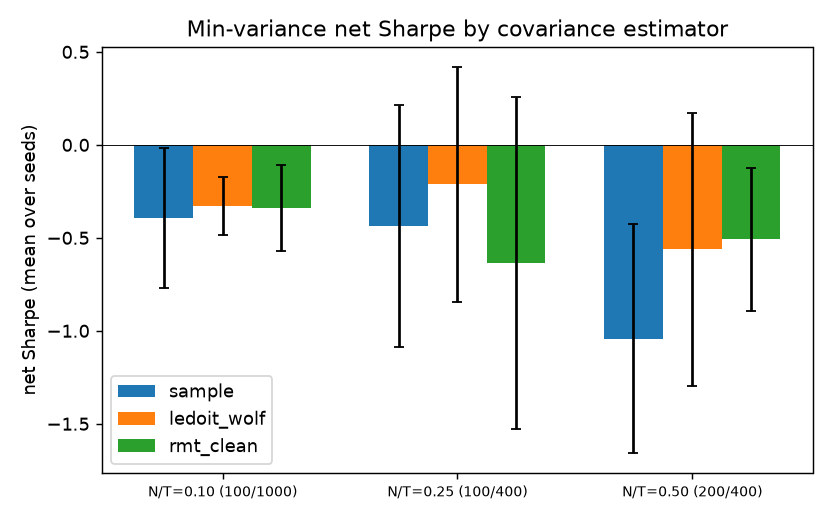
\includegraphics[keepaspectratio,alt={Net Sharpe by estimator across N/T regimes. Error bars: \$\$1 std over 5 seeds. The sample estimator degrades fastest as N/T grows; MP clipping and LW hold up.}]{sharpe_by_seed.png}}
\caption{Net Sharpe by estimator across N/T regimes. Error bars:
\$\pm\$1 std over 5 seeds. The sample estimator degrades fastest as N/T
grows; MP clipping and LW hold up.}
\end{figure}

\begin{figure}
\centering
\pandocbounded{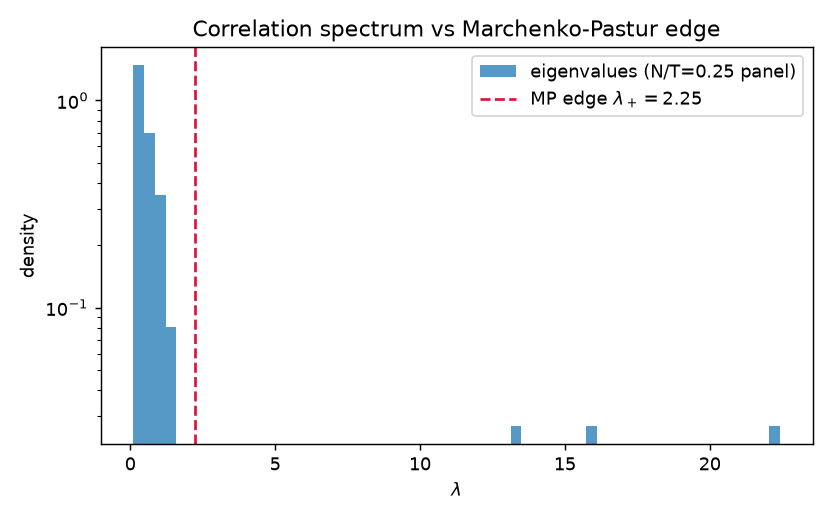
\includegraphics[keepaspectratio,alt={Correlation spectrum of a representative panel against the MP edge: the bulk fills the MP support while a handful of factor eigenvalues sit far above it --- exactly the structure the clipping rule assumes.}]{eigen_spectrum.png}}
\caption{Correlation spectrum of a representative panel against the MP
edge: the bulk fills the MP support while a handful of factor
eigenvalues sit far above it --- exactly the structure the clipping rule
assumes.}
\end{figure}

\textbf{Reading.} The ordering flips with \(N/T\) exactly as theory
predicts. When data are plentiful relative to assets (\(q = 0.1\)), the
sample covariance is nearly sufficient and all estimators tie. At
\(q = 0.5\) the sample covariance is 50\%-rank-deficient noise and the
cleaned variants halve its Sharpe penalty. The \(q = 0.25\) midpoint
favors LW --- consistent with LW's shrinkage target being tuned for
exactly this moderate-noise regime, while hard clipping discards some
genuine low-eigenvalue signal.

Absolute Sharpe levels are negative everywhere and \emph{should be}: the
DGP has zero alpha, so net Sharpe measures cost drag and variance
reduction, not skill. The comparison across estimators is the object of
study, not the level.

\section{4. Limitations}\label{limitations}

\begin{enumerate}
\def\labelenumi{\arabic{enumi}.}
\tightlist
\item
  Synthetic factor panels: the DGP's spherical idio noise is the best
  case for MP theory; real panels with heteroskedasticity and
  time-varying correlations will degrade clipping less predictably.
\item
  Five seeds: the seed-level std on Sharpe is \(\approx 0.3\); the
  \(q=0.5\) RMT-vs-sample gap (\(\approx 0.54\)) is \textasciitilde1.8
  seed-stds --- directionally solid, magnitude uncertain. The paired
  bootstrap on return streams is the sharper instrument and is reported
  per scenario.
\item
  GMV only; mean-variance with a signal model would reward covariance
  cleaning differently.
\item
  Hard clipping only; nonlinear shrinkage (Donoho--Gavish--Johnstone) is
  the documented next rung.
\end{enumerate}

\section{Reproducibility}\label{reproducibility}

\begin{verbatim}
pip install -e ".[dev]"
make test
python scripts/run_study.py          # regenerates every number and figure
\end{verbatim}
